\chapter{INTRODUCTION}

\subsection{The Primary Visual Cortex and the Limits of Static Topologies}
The primary visual cortex has long served as the canonical model for understanding cortical microcircuitry, sensory processing, and the brain's \textbf{neural networks}. Historically, the architectural and functional parcellation of visual areas---such as Area 17 (A17), Area 18 (A18), and their Transition Zone (TZ) in the feline model---has been extensively mapped using single-unit recordings and static receptive field analyses (Wunderle et al., 2013; Schmidt et al., 2023). These classical approaches have established the foundational \textbf{static connectome}---a rigid, structural blueprint of the visual system detailing how intra- and inter-hemispheric neural networks form clustered functional communities. 
\begin{figure}[htbp]
    \centering
    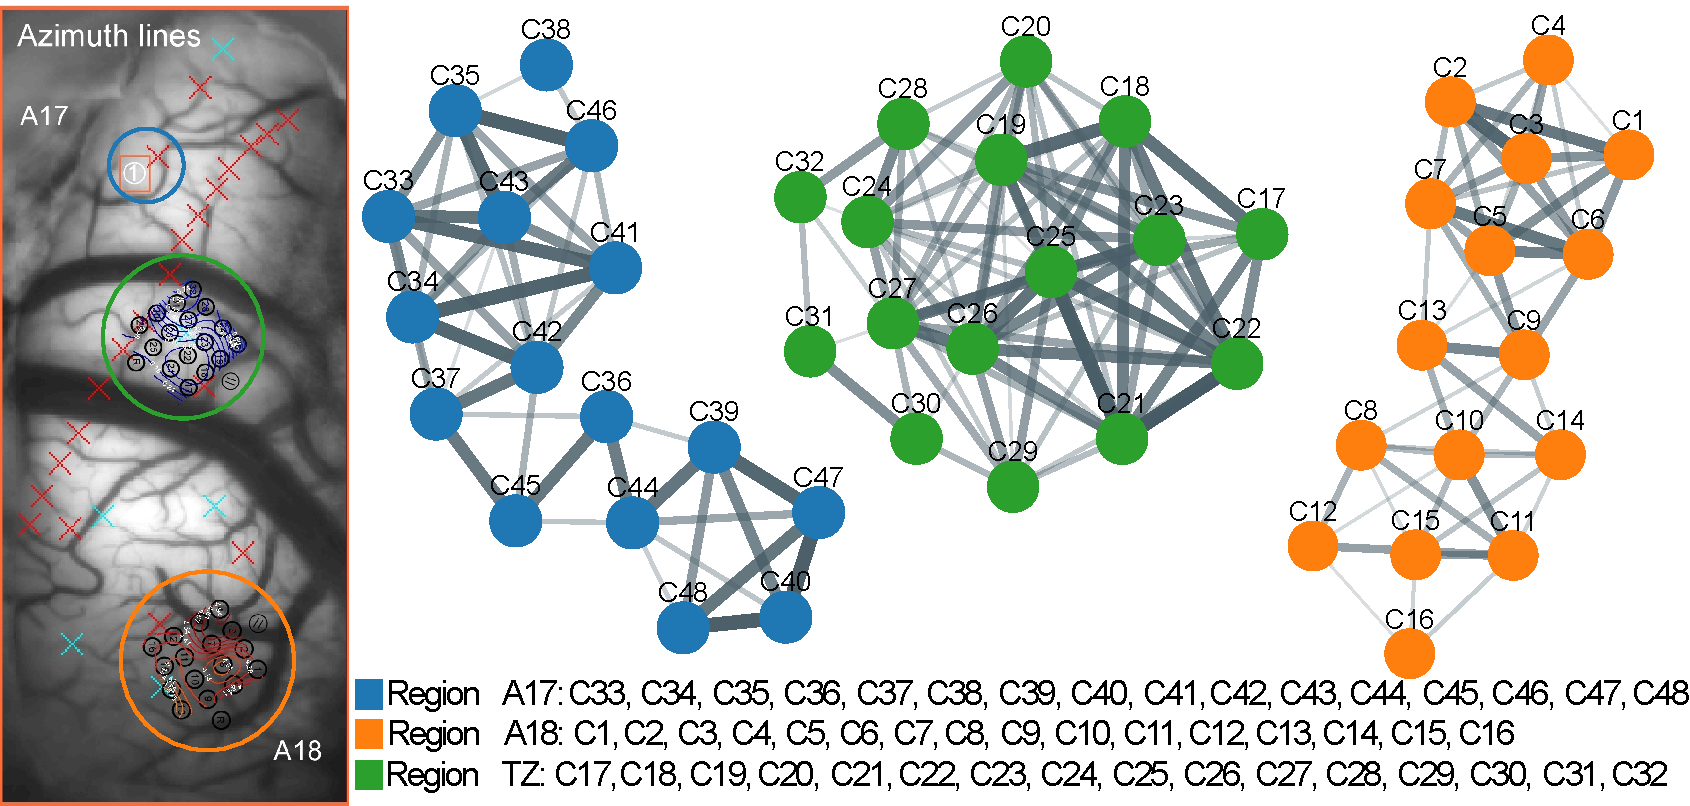
\includegraphics[width=\linewidth]{./figuras/Intro/Figura01.pdf}
    \caption[Mapping directly to the anatomically separated electrode matrixes]{\textbf{Mapping directly to the anatomically separated electrode matrixes | (Coherence (Low Gamma)) | Density: 15\%: Coherence clusters}}
    \label{fig:cortical_model}
\end{figure}
However, relying exclusively on these stationary statistical relationships collapses the true, living matrix of cortical connections. Averaging neural interactions over long temporal windows (e.g., minutes of recording) treats the neural network as a fixed roadmap, inevitably obscuring sub-second synaptic recruitment and leading to a severe loss of organic causality resolution. Cognitive processes, particularly visual feature binding, do not operate in a stationary state; they evolve dynamically and transiently as stimuli move across and between receptive fields. Consequently, \textbf{static topologies}---while accurately describing the anatomical constraints and the baseline connectome of neural communication---completely mask the rapid, transient fluctuations in functional integration that are the actual hallmark of active sensory processing.


\section{The Paradigm Shift to the "Dynome"}
To overcome the limitations of static connectomics, the neuroscientific community has begun shifting its focus toward the exploration of the "Dynome"—the millisecond-scale evolution of functional networks and their temporal dynamics \cite{kopell2014}. Capturing the Dynome requires shifting the analytical framework from time-averaged correlations to time-resolved state transitions, often achieved through sliding-window approaches \cite{allen2014}. By dissecting the continuous data stream into granular temporal epochs, it becomes possible to observe how network metrics, such as \textit{Small-Worldness} and modularity, adapt and evolve. This time-varying perspective provides a much more accurate representation of the brain's real-time functional state, revealing that macroscopic efficiency is not fixed but reacts continuously to ongoing sensory integration.

\section{Rhythmic Oscillations, Predictive Coding, and Gamma Synchronization}
At the mesoscopic scale, rhythmic neural oscillations—specifically in the Gamma frequency band (30–90 Hz)—act as a fundamental mechanism for cortical communication and information routing. Under the predictive coding framework, the synchronized engagement of neuronal populations in the gamma band provides a fast transmission channel for feedforward visual processing, carrying sensory "prediction errors" from primary areas (A17) to higher-order regions (A18) \cite{vezoli2021}. Furthermore, the Transition Zone (TZ) acts not merely as a geographic boundary, but as a highly specialized region densely innervated by transcallosal projections, facilitating massive interhemispheric coordination essential for integrating visual stimuli across the vertical meridian \cite{schmidt2023}. Thus, mapping the directionality of gamma synchronization across A17, TZ, and A18 is crucial for deciphering the causal architecture and dynamic modulation of the visual cortex.

\section{The Methodological Bottleneck in Electrophysiology}
Despite the theoretical necessity of time-resolved, directed connectivity analysis, extracting these networks from dense multi-electrode arrays poses severe methodological and computational challenges. The primary analytical bottleneck in Local Field Potential (LFP) analysis is \textit{volume conduction}—the instantaneous spread of electrical fields through cortical tissue. This phenomenon causes multiple electrodes to record a single biological source simultaneously, generating spurious zero-phase lag correlations that heavily contaminate graph topologies with false-positive edges \cite{bastos2015}.

Furthermore, the transition to high-density electrophysiology (e.g., 32-64 channel matrices) creates a "Big Data" computational crisis. Calculating dynamic, non-linear connectivity metrics (such as Partial Directed Coherence or phase-based indices), generating hundreds of surrogate networks for statistical validation, and tracking graph properties over moving time windows inevitably lead to combinatorial explosions. Traditional, single-threaded analytical scripts are inherently incapable of managing such stochastic, multidimensional loads, often resulting in Out-of-Memory (OOM) failures or prohibitive processing times. 

Consequently, there is a critical need for a modern, high-performance computing (HPC) framework capable of mitigating volume conduction artifacts through advanced phase-based estimators while leveraging distributed parallel processing to interactively render the mesoscopic Dynome.

\vspace{1cm}

% --- VISUAL INSERTION USING TIKZ ---
\begin{figure}[htbp]
    \centering
    \begin{tikzpicture}[
        box/.style={draw, rounded corners, minimum width=2.5cm, minimum height=1cm, align=center, fill=blue!5, font=\sffamily\small},
        circ/.style={draw, circle, minimum size=1.5cm, align=center, fill=red!5, font=\sffamily\small},
        >={Stealth},
        thick
    ]
        
        % ================= PANEL A =================
        \node[font=\bfseries\sffamily] at (0, 0) {Painel A: Condução de Volume vs. Resolução Analítica};
        
        % Volume Conduction Side
        \node[circ] (dipole) at (-4, -2) {Deep\\Dipole};
        \node[box] (e1) at (-7, -5) {CH 1};
        \node[box] (e2) at (-4.5, -5) {CH 2};
        \node[box] (e3) at (-2, -5) {CH 3};
        \node[box] (e4) at (0.5, -5) {CH 4};
        
        \draw[->, dashed] (dipole) -- (e1);
        \draw[->, dashed] (dipole) -- (e2);
        \draw[->, dashed] (dipole) -- (e3);
        \draw[->, dashed] (dipole) -- (e4);
        
        \draw[<->, red] (e1) to[bend right=25] node[below, font=\scriptsize\sffamily] {Zero-lag} (e2);
        \draw[<->, red] (e2) to[bend right=25] (e3);
        \draw[<->, red] (e3) to[bend right=25] (e4);
        \draw[<->, red] (e1) to[bend right=40] (e4);
        
        % Filter Side
        \node[box, fill=orange!10, minimum height=1.5cm] (filter) at (4, -2.5) {Complex Domain\\Filter\\(wPLI / iCoh)};
        
        \node[circ, fill=green!10] (n1) at (2.5, -5) {Node 1};
        \node[circ, fill=green!10] (n3) at (5.5, -5) {Node 3};
        
        \draw[->, ultra thick] (e4.east) to[out=0, in=180] (filter.west);
        \draw[->, ultra thick] (filter.south) -- (4, -3.8) -| (n1.north);
        \draw[->, ultra thick] (filter.south) -- (4, -3.8) -| (n3.north);
        
        \draw[<->, ultra thick, green!50!black] (n1) -- node[above, font=\scriptsize\sffamily] {Valid Edge} (n3);
        
        
        % ================= PANEL B =================
        \node[font=\bfseries\sffamily] at (0, -8.5) {Painel B: Colapso Temporal vs. Dinoma Transiente};
        
        % Static Approach
        \node[box] (t1) at (-5.5, -10) {State 1};
        \node[box] (t2) at (-2.5, -10) {State 2};
        \node[box] (t3) at (0.5, -10) {State 3};
        
        \node[circ, fill=orange!10] (avg) at (-2.5, -12.5) {Long Window\\Average};
        \draw[->] (t1) -- (avg);
        \draw[->] (t2) -- (avg);
        \draw[->] (t3) -- (avg);
        
        \node[box, fill=red!10, minimum width=4cm] (dense) at (-2.5, -15) {Dense, Unrealistic\\Static Graph};
        \draw[->] (avg) -- (dense);
        
        % Dynamic Approach
        \node[circ, fill=green!10] (g1) at (4.5, -10) {Engram 1};
        \node[circ, fill=green!10] (g2) at (4.5, -12.5) {Engram 2};
        \node[circ, fill=green!10] (g3) at (4.5, -15) {Engram 3};
        
        \draw[->, blue, dashed, ultra thick] (g1) -- node[right, font=\scriptsize\sffamily] {Temporal flexibility} (g2);
        \draw[->, blue, dashed, ultra thick] (g2) -- (g3);
        
        % connecting visual
        \draw[->, dotted, thick, gray] (t3.east) to[out=0, in=180] node[above, font=\scriptsize\sffamily] {Dynome View} (g1.west);
        
    \end{tikzpicture}
    
    \caption[Esquematização dos gargalos metodológicos]{\textbf{Esquematização dos principais gargalos metodológicos em conectômica eletrofisiológica e suas respectivas resoluções no framework proposto.} \textbf{(Painel A)} Representação biofísica da Condução de Volume: as linhas de campo elétrico de um único dipolo profundo atingem instantaneamente múltiplos microeletrodos, criando anomalias de \textit{zero-lag} e gerando matrizes topológicas falsamente densas. À direita, a resolução analítica utilizando índices de fase complexa (wPLI/iCoh), que filtra os artefatos e recupera um grafo esparso e fidedigno. \textbf{(Painel B)} Representação abstrata do colapso temporal: o cálculo de correlações através de janelas demasiadamente longas funde diferentes estados cerebrais transitórios, resultando numa rede artificial estática. Em contraste, a exploração focada no ``Dinoma'' preserva a flexibilidade sequencial e as rápidas reorganizações dos engramas funcionais de integração.}
    \label{fig:methodological_bottlenecks}
\end{figure}